
\documentclass{beamer}
\usecolortheme{dove}
\setbeamertemplate{navigation symbols}{}
\usepackage{amsmath,amssymb,amsfonts,amsthm, multicol, subfigure, color}
\usepackage{bm}
\usepackage{graphicx}
\usepackage{tabularx}
\usepackage{booktabs}
\usepackage{hyperref}
\usepackage{pdfpages}
\usepackage{xcolor}
\definecolor{seagreen}{RGB}{46, 139, 87}
\def\independenT#1#2{\mathrel{\rlap{$#1#2$}\mkern2mu{#1#2}}}
\newcommand\indep{\protect\mathpalette{\protect\independenT}{\perp}}
\def\log{\text{log}}
\newcommand\logit{\text{logit}}
\newcommand\iid{\stackrel{\text{iid}}{\sim}}
\newcommand\E{\text{E}}
\newcommand\V{\text{V}}
\renewcommand\P{\text{P}}
\newcommand{\Cov}{\text{Cov}}
\newcommand{\Cor}{\text{Cor}}
\newcommand\doop{\texttt{do}}
\usepackage{stackrel}
\usepackage{tikz}
\usetikzlibrary{arrows,shapes.arrows,positioning,shapes,patterns,calc}
\newcommand\slideref[1]{\vskip .1cm \tiny \textcolor{gray}{{#1}}}
\newcommand\red[1]{\color{red}#1}
\newcommand\blue[1]{\color{blue}#1}
\newcommand\gray[1]{\color{gray}#1}
\newcommand\seagreen[1]{\color{seagreen}#1}
\newcommand\purple[1]{\color{purple}#1}
\newcommand\orange[1]{\color{orange}#1}
\newcommand\black[1]{\color{black}#1}
\newcommand\white[1]{\color{white}#1}
\newcommand\teal[1]{\color{teal}#1}
\newcommand\magenta[1]{\color{magenta}#1}
\newcommand\Fuchsia[1]{\color{Fuchsia}#1}
\newcommand\BlueGreen[1]{\color{BlueGreen}#1}
\newcommand\bblue[1]{\textcolor{blue}{\textbf{#1}}}
\newcommand\bred[1]{\textcolor{red}{\textbf{#1}}}
\newcommand\bgray[1]{\textcolor{gray}{\textbf{#1}}}
\newcommand\bgreen[1]{\textcolor{seagreen}{\textbf{#1}}}
\newcommand\bref[2]{\href{#1}{\color{blue}{#2}}}
\colorlet{lightgray}{gray!40}
\pgfdeclarelayer{bg}    % declare background layer for tikz
\pgfsetlayers{bg,main} % order layers for tikz
\newcommand\mycite[1]{\begin{scriptsize}\textcolor{darkgray}{(#1)}\end{scriptsize}}
\newcommand{\tcframe}{\frame{
%\small{
\only<1|handout:0>{\tableofcontents}
\only<2|handout:1>{\tableofcontents[currentsubsection]}}
%}
}

\newcommand{\goalsframe}{\begin{frame}{Learning goals for today}
By the end of class, you will be able to
\begin{itemize}
    \item use statistical learning to estimate when data are sparse
    \item work with models that are ``wrong''
 \end{itemize} 
  \vskip .2in
\end{frame}}

\newcommand{\credible}{\begin{frame}{Credible science}
\begin{enumerate}
\item replicability
\item reproducibility
\end{enumerate}
\end{frame}}

\usepackage[round]{natbib}
\bibliographystyle{humannat-mod}
\setbeamertemplate{enumerate items}[default]
\usepackage{mathtools}

\title{Studying Social Inequality with Data Science}
\author{Ian Lundberg}
\date{\today}

\begin{document}

\begin{frame}
\begin{tikzpicture}[x = \textwidth, y = \textheight]
\node at (0,0) {};
\node at (1,1) {};
\node[anchor = north west, align = left, font = \huge] at (0,.9) {Studying\\Social Inequality\\with Data Science};
\node[anchor = north east, align = right] (number) at (1,.9) {INFO 3370 / 5371\\Spring 2024};
\node[anchor = north, font = \Large, align = center] at (.5,.5) {Statistical Learning};
\end{tikzpicture}
\end{frame}

\goalsframe

\begin{frame}

{\huge statistical learning: the idea} \vskip .2in
illustrated by a
\begin{itemize}
\item discrete numeric predictor
\item continuous numeric predictor
\end{itemize}
\end{frame}

% ESTIMATE AN AVERAGE GIVEN X

\begin{frame}%{Statistical learning from samples}

With only the sample, how would you estimate the mean salary of all the Dodgers? \vskip .2in

\begin{tabular}{ll}
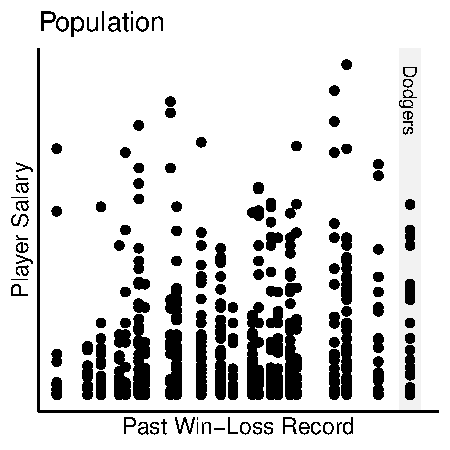
\includegraphics[width = .48\textwidth]{dodgers_population} &
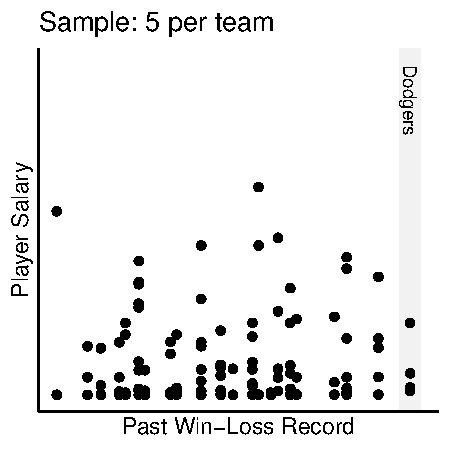
\includegraphics[width = .48\textwidth]{dodgers_sample}
\end{tabular}

\end{frame}

\begin{frame}{Three estimators for the Dodgers' mean salary}

\includegraphics<1>[width = \textwidth]{dodgers_estimator1}
\includegraphics<2>[width = \textwidth]{dodgers_estimator2}
\includegraphics<3>[width = \textwidth]{dodgers_estimator3}
\only<4->{
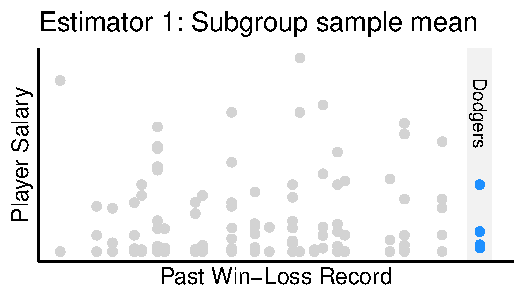
\includegraphics[width = .32\textwidth]{dodgers_estimator1}
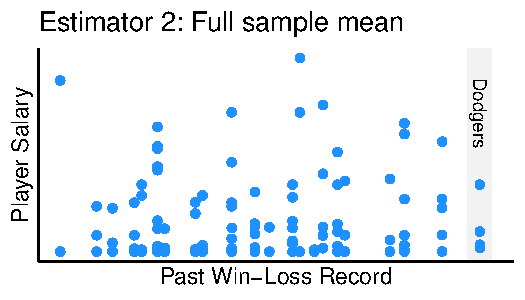
\includegraphics[width = .32\textwidth]{dodgers_estimator2}
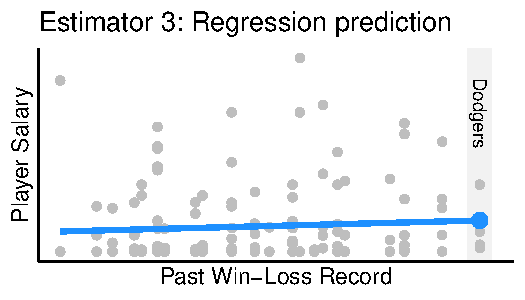
\includegraphics[width = .32\textwidth]{dodgers_estimator3} \vskip .2in
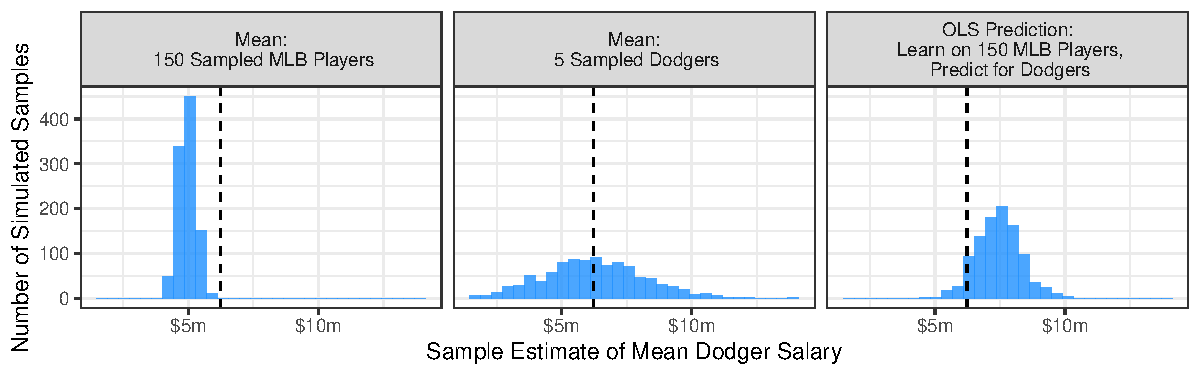
\includegraphics[width = \textwidth]{dodgers_estimator_histogram} \vskip .2in
\onslide<5->{
Which do you prefer? Why is your choice a little weird?
}
}

\end{frame}

\begin{frame}{Statistical learning: A somewhat unusual view} \pause

\begin{enumerate}
\item the entire goal of modeling is to solve sparse data
\begin{itemize}
\item we sample very few Dodgers,\\so we use non-Dodgers to help our estimate
\end{itemize} \pause \vskip .1in
\item in a huge sample, a model is unnecessary
\begin{itemize}
\item estimate Dodger population mean\\by the Dodger sample mean
\end{itemize} \pause \vskip .1in
\item in a tiny sample, models may perform poorly
\begin{itemize}
\item might even better to estimate a subgroup mean (Dodgers)\\by taking the mean of the whole sample (all MLB)
\end{itemize}
\end{enumerate}

\end{frame}

\begin{frame}

{\huge statistical learning: the idea} \vskip .2in
illustrated by a
\begin{itemize}
\item discrete numeric predictor
\item continuous numeric predictor
\end{itemize}
\end{frame}

\begin{frame}

What is the mean 2023 salary among players\\who in 2021 earned \$5-10 million?

\end{frame}

% ESTIMATE AN AVERAGE OVER X

% SAMPLE MEAN STRATEGY
\begin{frame}{Goal: Estimate a target population mean from a sample}{Method: Sample subgroup mean}
\begin{tikzpicture}[x = \textwidth, y = \textheight]
\node at (0,0) {};
\node at (1,1) {};
\node<1>[anchor = north west] at (0,.9) {Begin with the population};
\node<1>[anchor = west] at (0,.5) {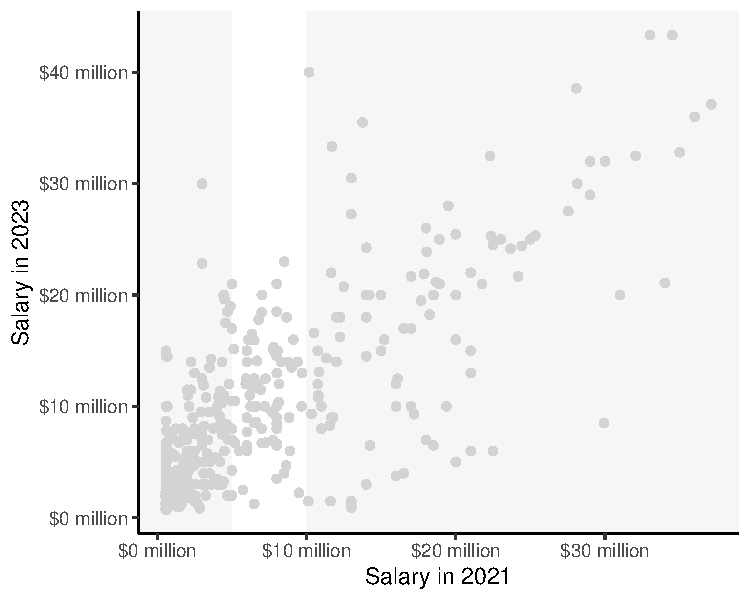
\includegraphics[width = .6\textwidth]{sims/population}};
\node<2->[anchor = north west] at (0,.9) {Sample};
\node<2>[anchor = west] at (0,.5) {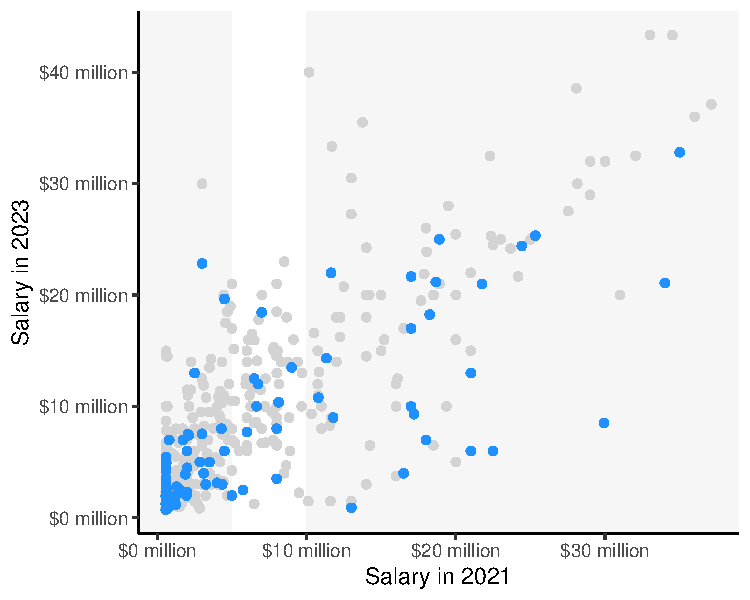
\includegraphics[width = .6\textwidth]{sims/sample_1}};
\node<5>[anchor = west] at (0,.5) {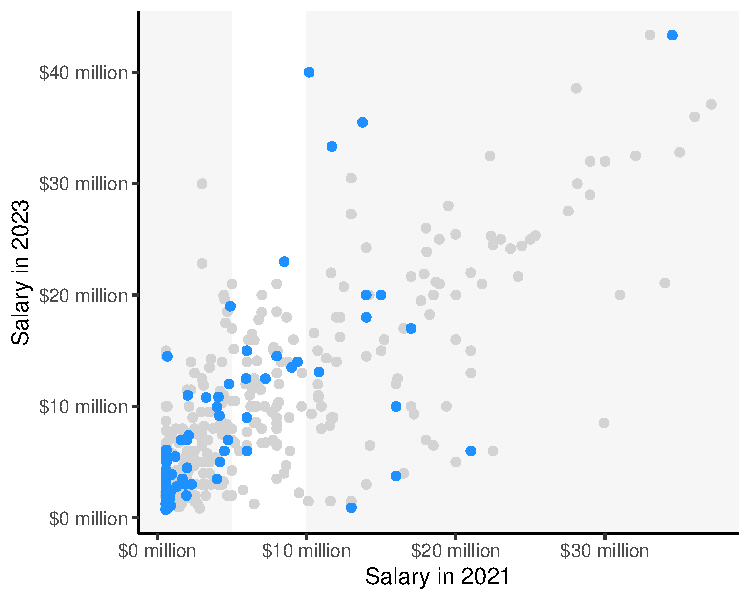
\includegraphics[width = .6\textwidth]{sims/sample_2}};
\node<8>[anchor = west] at (0,.5) {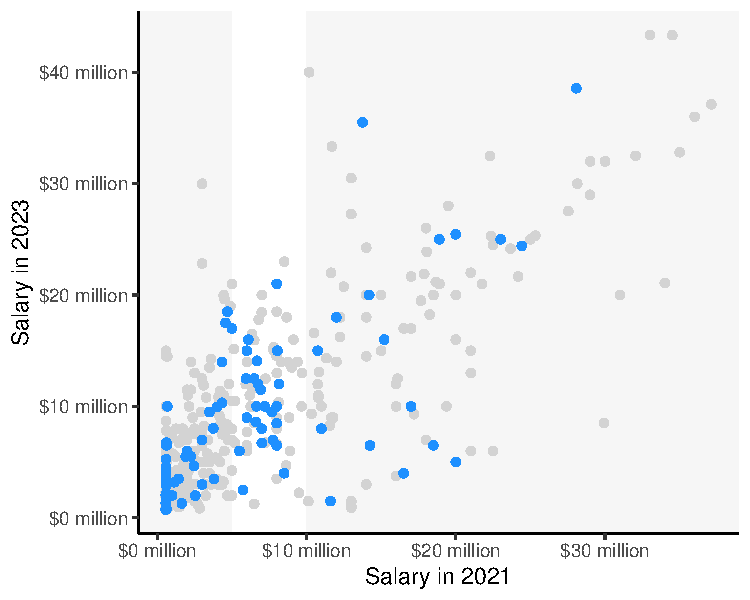
\includegraphics[width = .6\textwidth]{sims/sample_3}};
\node<3-4>[anchor = west] at (0,.5) {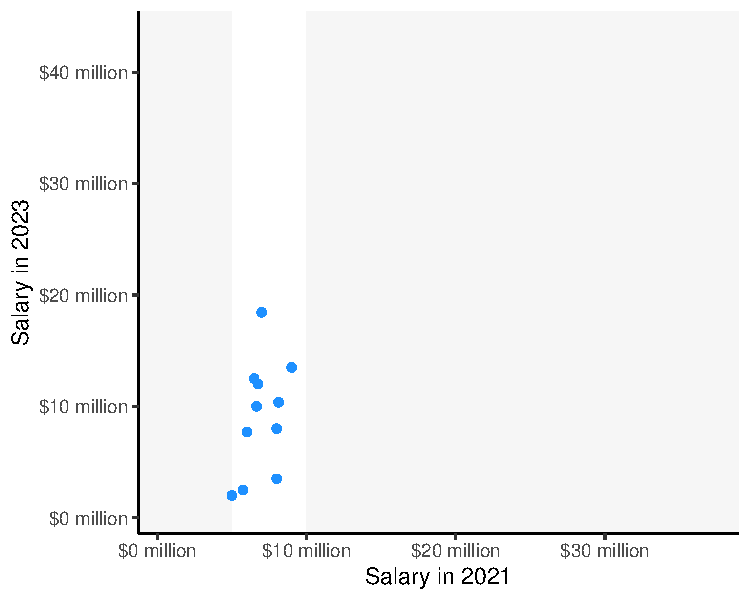
\includegraphics[width = .6\textwidth]{sims/mean_estimator_1}};
\node<6-7>[anchor = west] at (0,.5) {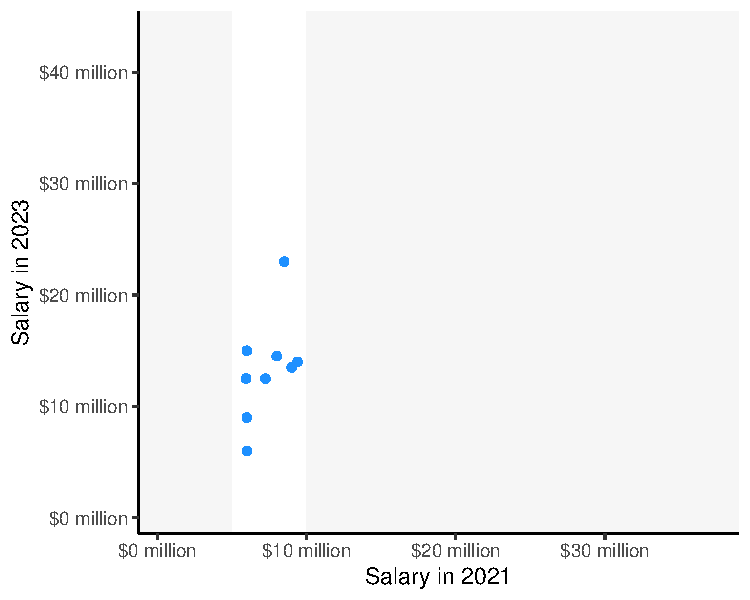
\includegraphics[width = .6\textwidth]{sims/mean_estimator_2}};
\node<9-10>[anchor = west] at (0,.5) {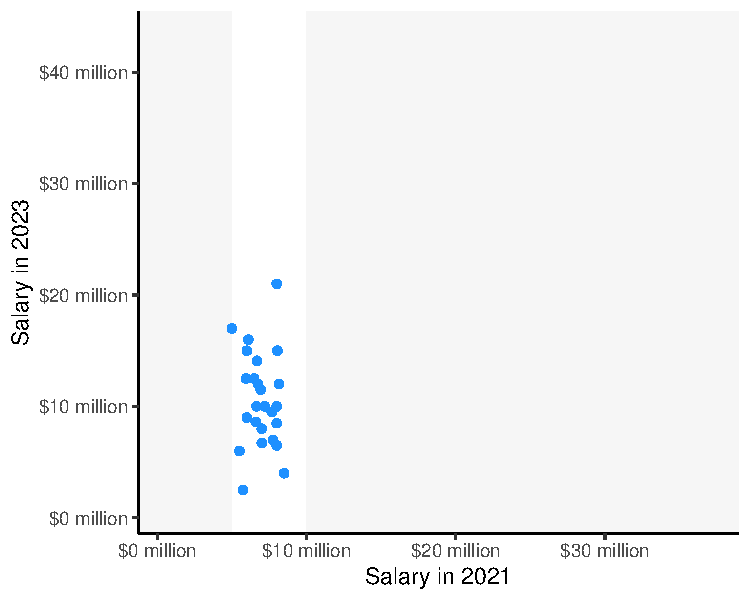
\includegraphics[width = .6\textwidth]{sims/mean_estimator_3}};
\node<11>[anchor = west] at (0,.5) {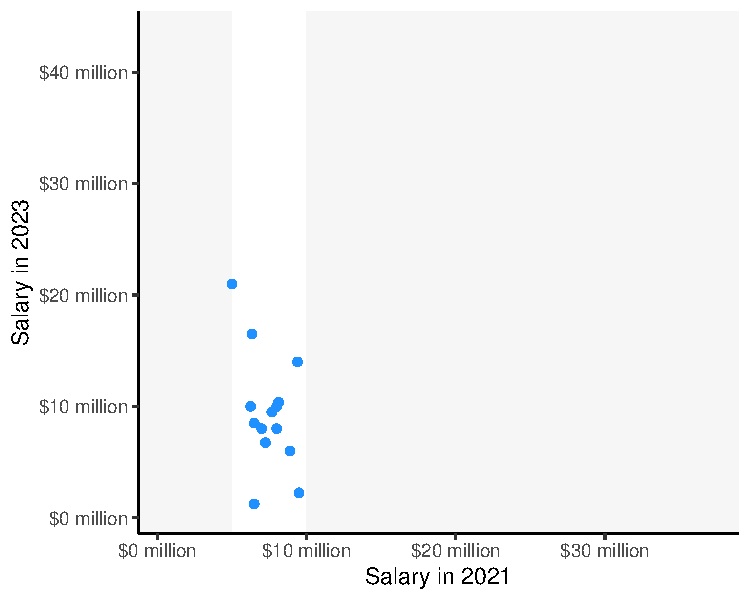
\includegraphics[width = .6\textwidth]{sims/mean_estimator_4}};
\node<12>[anchor = west] at (0,.5) {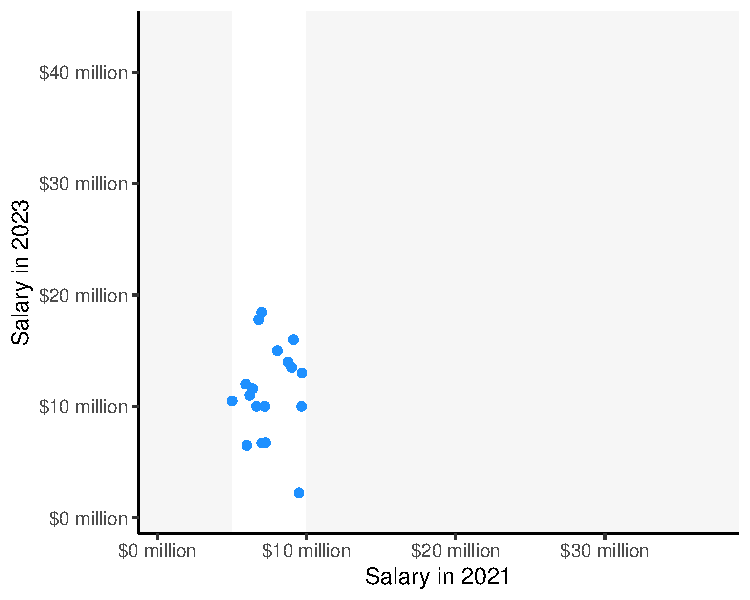
\includegraphics[width = .6\textwidth]{sims/mean_estimator_5}};
\node<13>[anchor = west] at (0,.5) {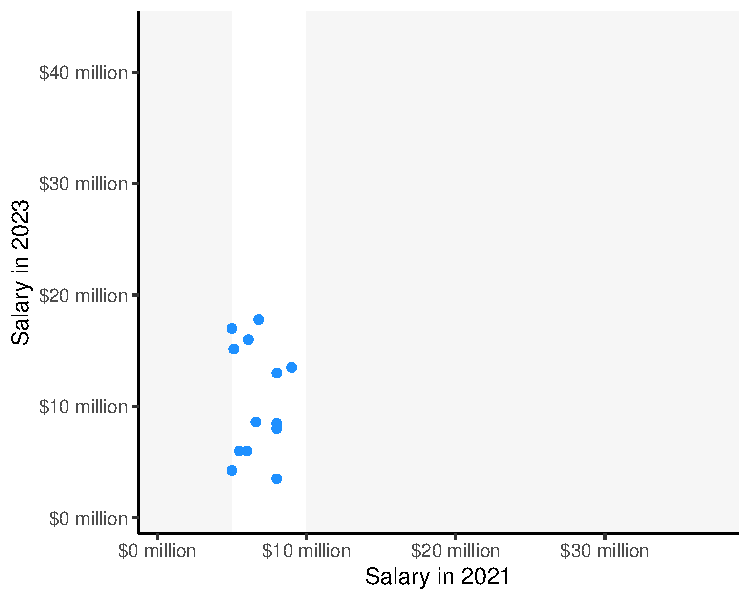
\includegraphics[width = .6\textwidth]{sims/mean_estimator_10}};
\node<14>[anchor = west] at (0,.5) {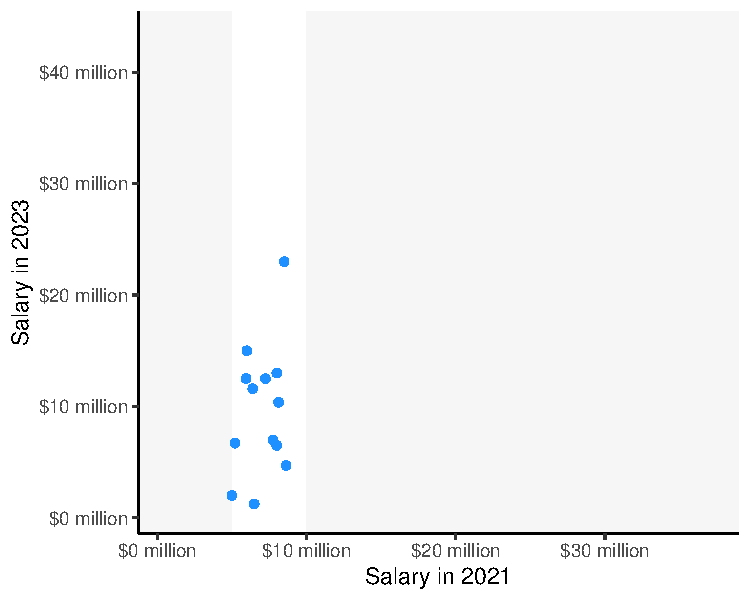
\includegraphics[width = .6\textwidth]{sims/mean_estimator_50}};
\node<15>[anchor = west] at (0,.5) {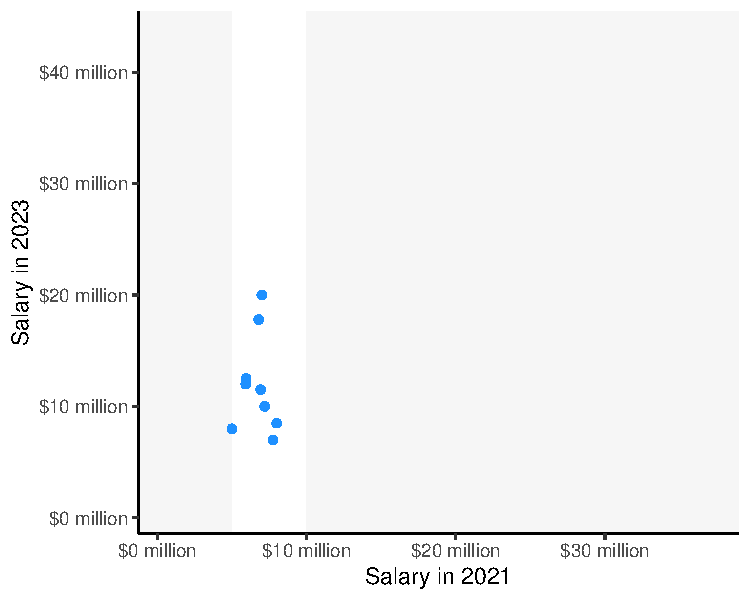
\includegraphics[width = .6\textwidth]{sims/mean_estimator_100}};
\node<4->[anchor = north east] at (1,.9) {Sample average};
\node<4-6>[anchor = east] at (1,.5) {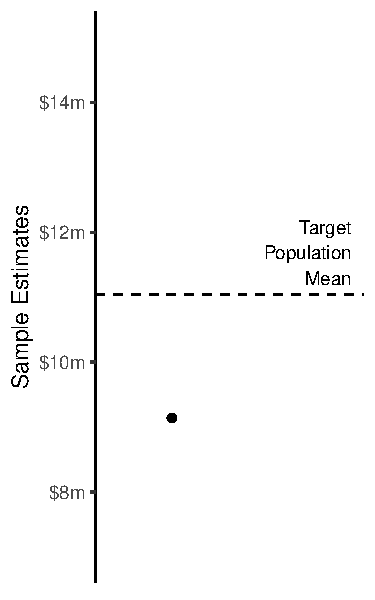
\includegraphics[width = .3\textwidth]{sims/mean_estimate_1}};
\node<7-9>[anchor = east] at (1,.5) {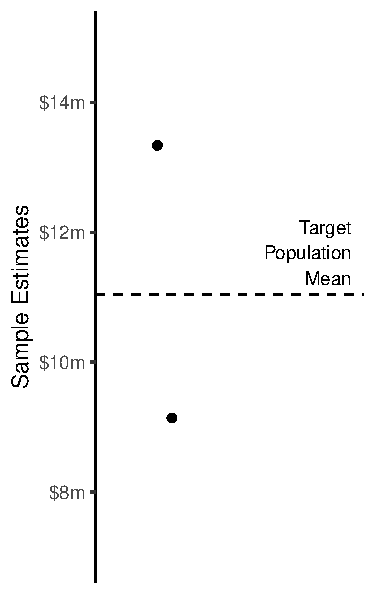
\includegraphics[width = .3\textwidth]{sims/mean_estimate_2}};
\node<10>[anchor = east] at (1,.5) {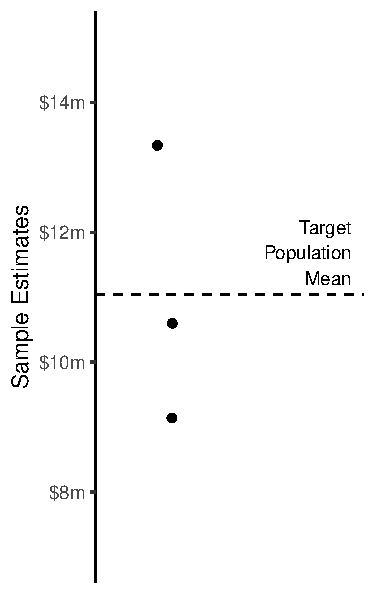
\includegraphics[width = .3\textwidth]{sims/mean_estimate_3}};
\node<11>[anchor = east] at (1,.5) {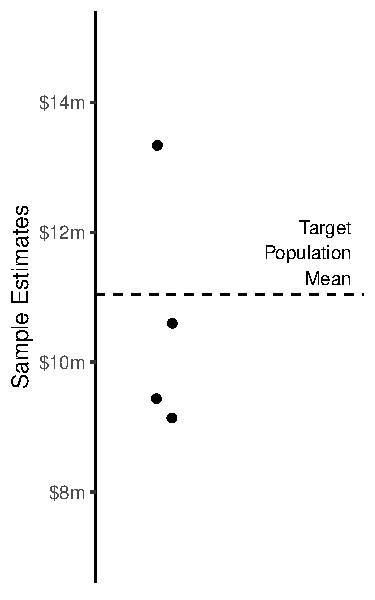
\includegraphics[width = .3\textwidth]{sims/mean_estimate_4}};
\node<12>[anchor = east] at (1,.5) {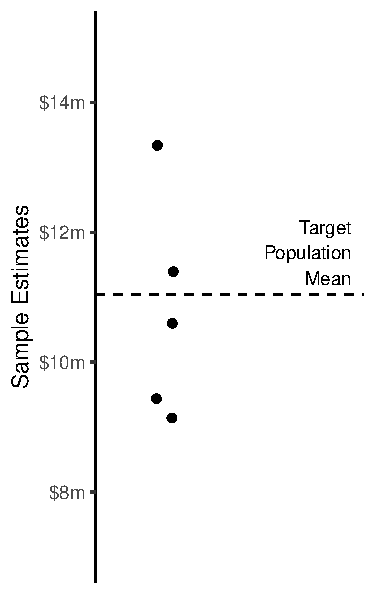
\includegraphics[width = .3\textwidth]{sims/mean_estimate_5}};
\node<13>[anchor = east] at (1,.5) {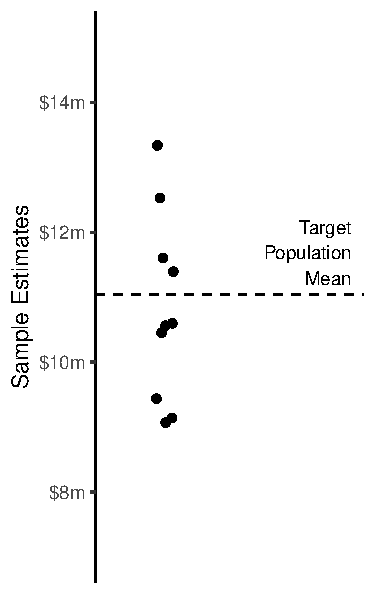
\includegraphics[width = .3\textwidth]{sims/mean_estimate_10}};
\node<14>[anchor = east] at (1,.5) {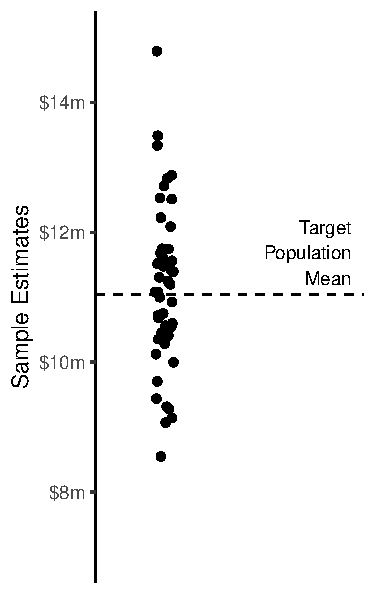
\includegraphics[width = .3\textwidth]{sims/mean_estimate_50}};
\node<15>[anchor = east] at (1,.5) {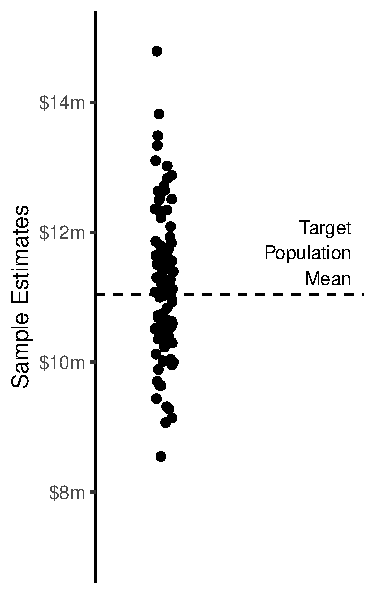
\includegraphics[width = .3\textwidth]{sims/mean_estimate_100}};
\end{tikzpicture}
\end{frame}

\begin{frame}{Goal: Estimate a target population mean from a sample}{Method: Ordinary Least Squares prediction}
\begin{tikzpicture}[x = \textwidth, y = \textheight]
\node at (0,0) {};
\node at (1,1) {};
\node<1>[anchor = north west] at (0,.9) {How would you use a model?};
\node<1>[anchor = west] at (0,.5) {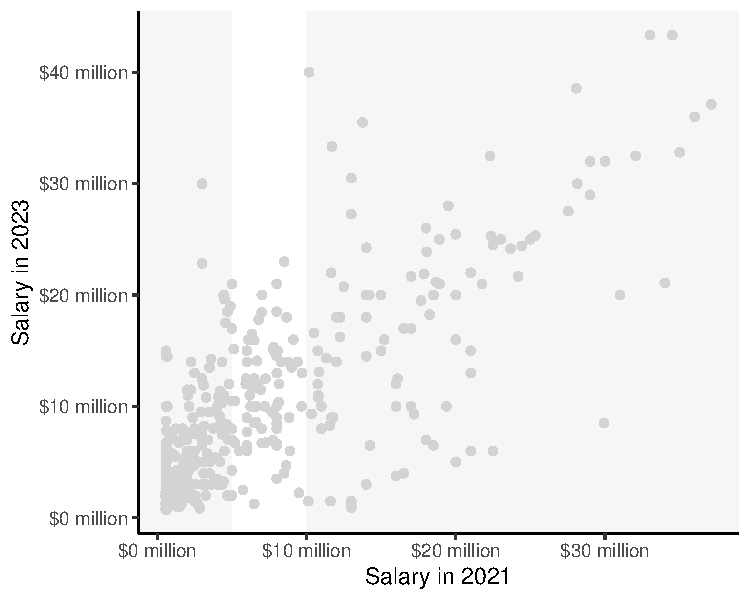
\includegraphics[width = .6\textwidth]{sims/population}};
\end{tikzpicture}
\end{frame}

% OLS SAMPLE 1
\begin{frame}{Goal: Estimate a target population mean from a sample}{Method: Ordinary Least Squares prediction}
\begin{tikzpicture}[x = \textwidth, y = \textheight]
\node at (0,0) {};
\node at (1,1) {};
\node<1>[anchor = north west] at (0,.9) {Begin with the population};
\node<1>[anchor = west] at (0,.5) {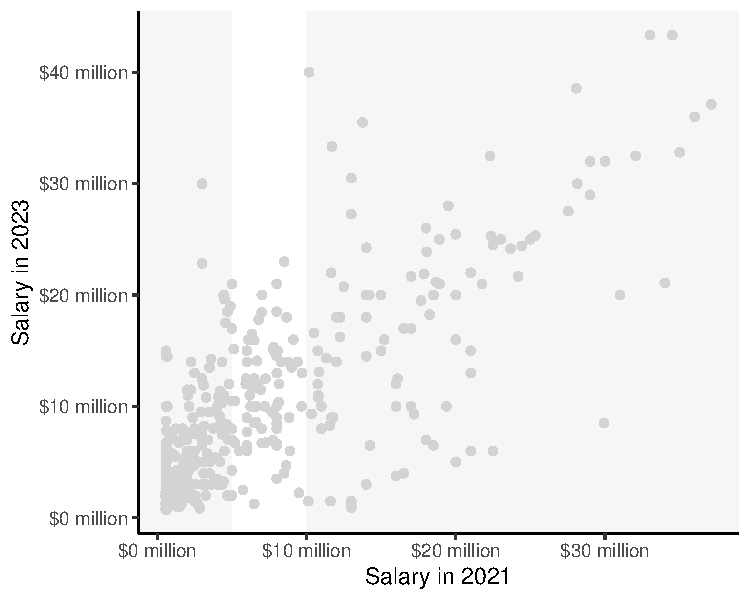
\includegraphics[width = .6\textwidth]{sims/population}};
\node<2>[anchor = north west] at (0,.9) {Draw a sample};
\node<2>[anchor = west] at (0,.5) {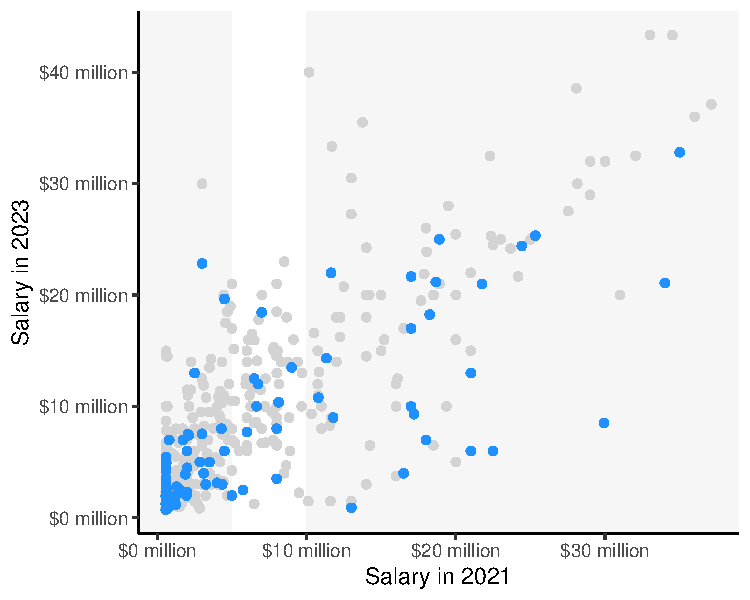
\includegraphics[width = .6\textwidth]{sims/sample_1}};
\node<3>[anchor = north west] at (0,.9) {Learn a model};
\node<3>[anchor = west] at (0,.5) {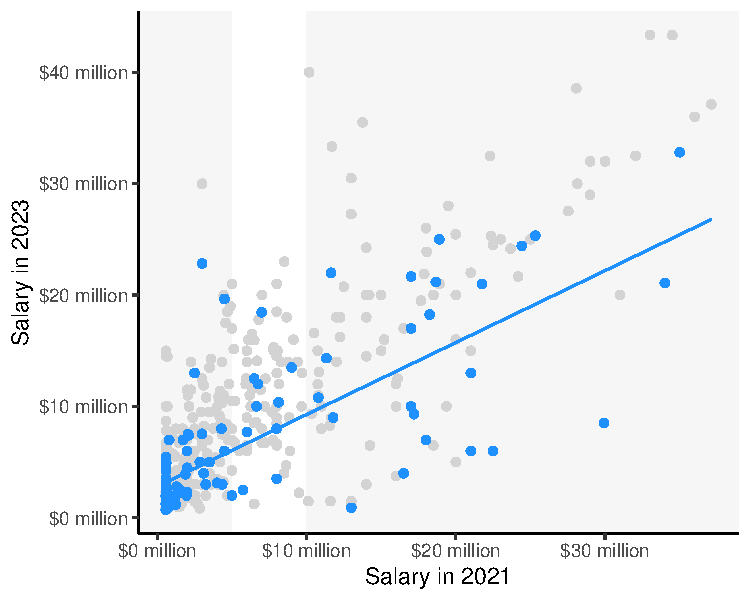
\includegraphics[width = .6\textwidth]{sims/ols_fit_1}};
\node<4>[anchor = north west] at (0,.9) {Focus on the target population};
\node<4>[anchor = west] at (0,.5) {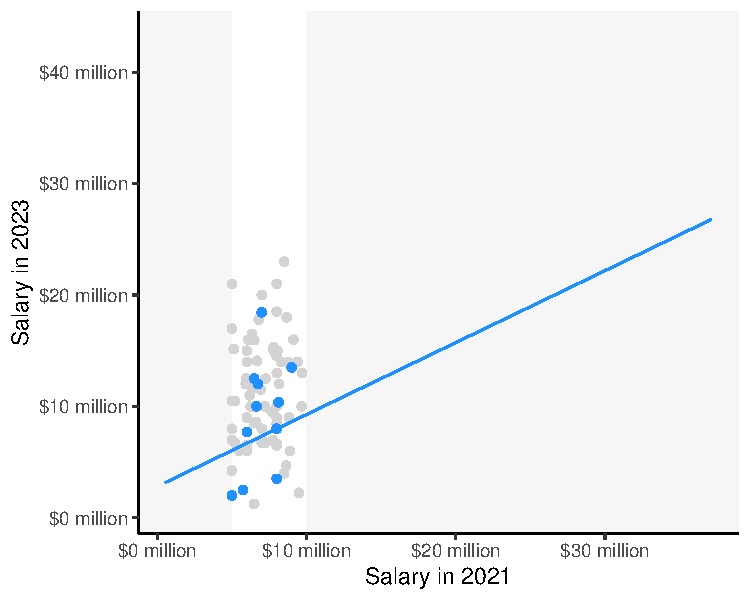
\includegraphics[width = .6\textwidth]{sims/ols_target_1}};
\node<5-6>[anchor = west] at (0,.5) {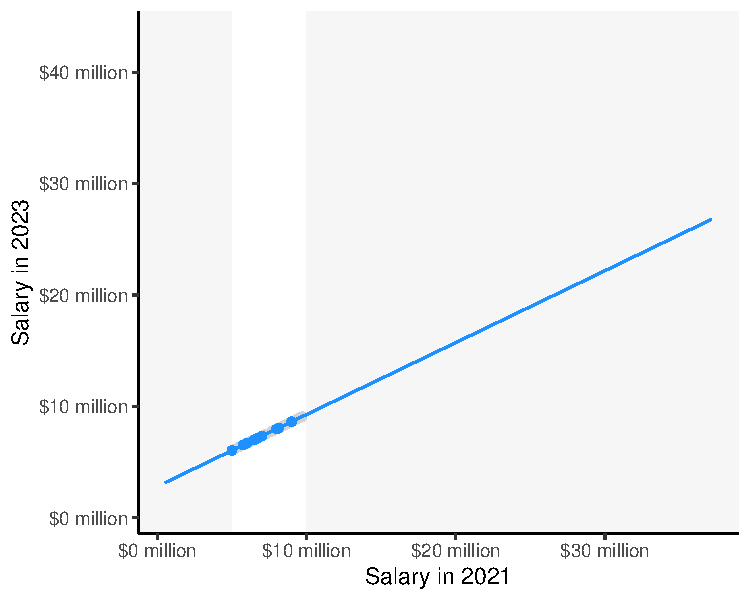
\includegraphics[width = .6\textwidth]{sims/ols_predicted_1}};
\node<5-6>[anchor = north west] (predict) at (0,.9) {Predict};
\node<6>[anchor = north east] at (1,.9) {Record the average};
\node<6>[anchor = east] at (1,.5) {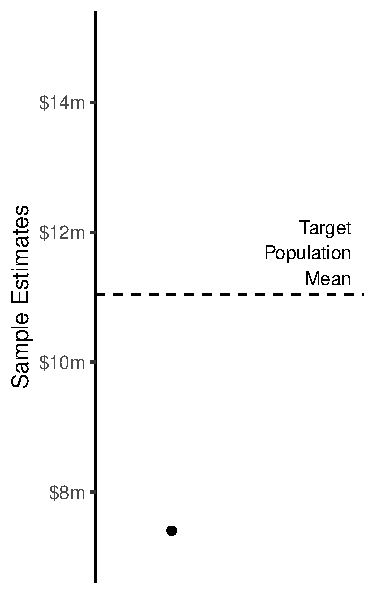
\includegraphics[width = .3\textwidth]{sims/ols_estimate_1}};
\end{tikzpicture}
\end{frame}
% OLS SAMPLE 2
\begin{frame}{Goal: Estimate a target population mean from a sample}{Method: Ordinary Least Squares prediction}
\begin{tikzpicture}[x = \textwidth, y = \textheight]
\node at (0,0) {};
\node at (1,1) {};
\node<1>[anchor = north west] at (0,.9) {Begin with the population};
\node<1>[anchor = west] at (0,.5) {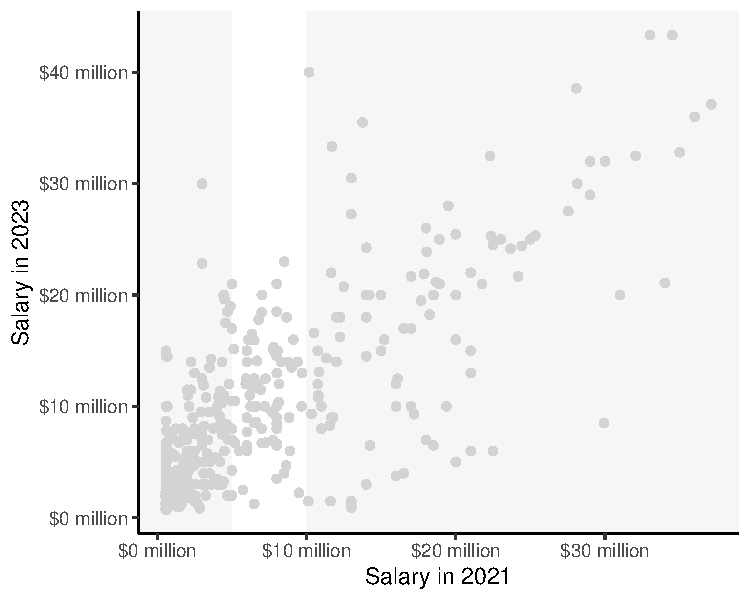
\includegraphics[width = .6\textwidth]{sims/population}};
\node<2>[anchor = north west] at (0,.9) {Draw a sample};
\node<2>[anchor = west] at (0,.5) {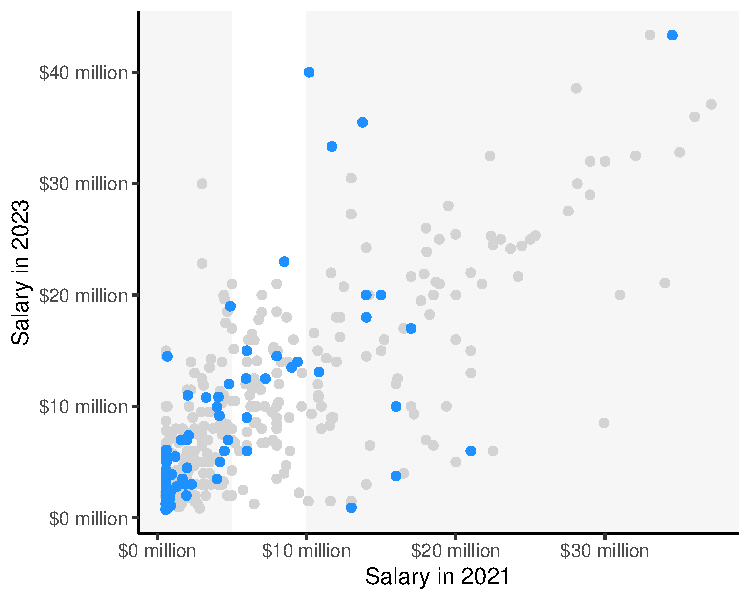
\includegraphics[width = .6\textwidth]{sims/sample_2}};
\node<3>[anchor = north west] at (0,.9) {Learn a model};
\node<3>[anchor = west] at (0,.5) {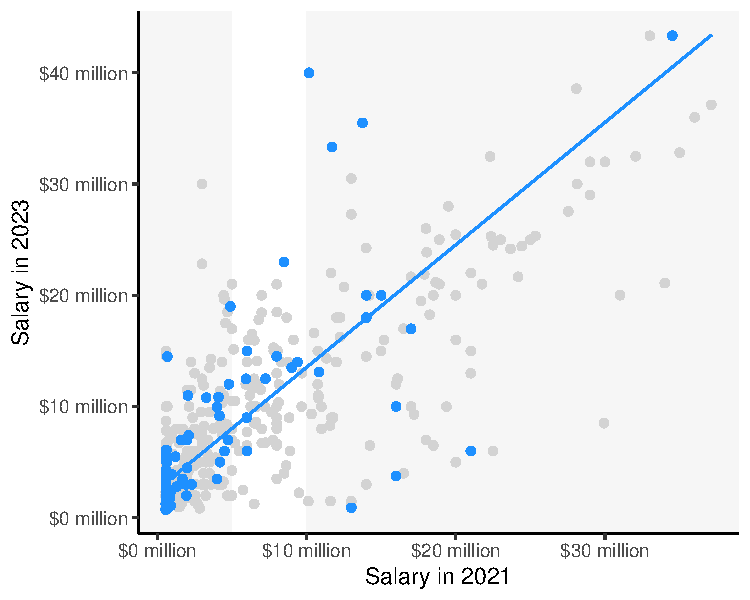
\includegraphics[width = .6\textwidth]{sims/ols_fit_2}};
\node<4>[anchor = north west] at (0,.9) {Focus on the target population};
\node<4>[anchor = west] at (0,.5) {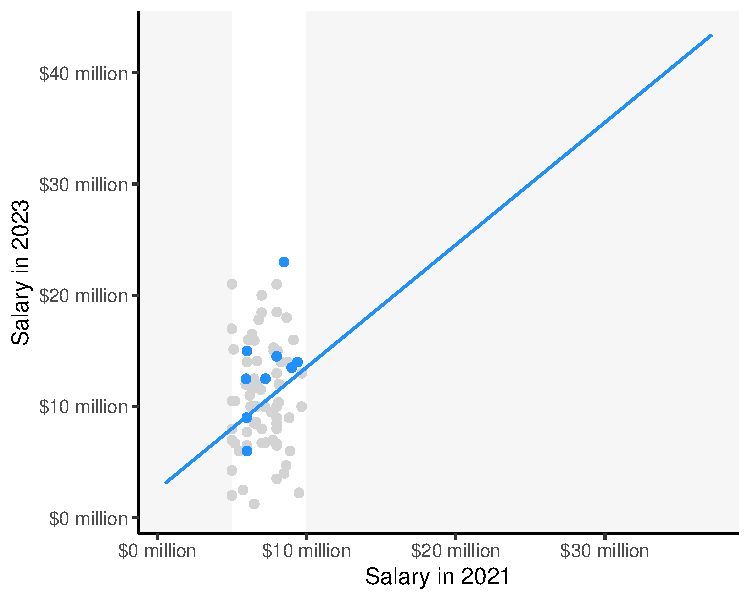
\includegraphics[width = .6\textwidth]{sims/ols_target_2}};
\node<5-6>[anchor = west] at (0,.5) {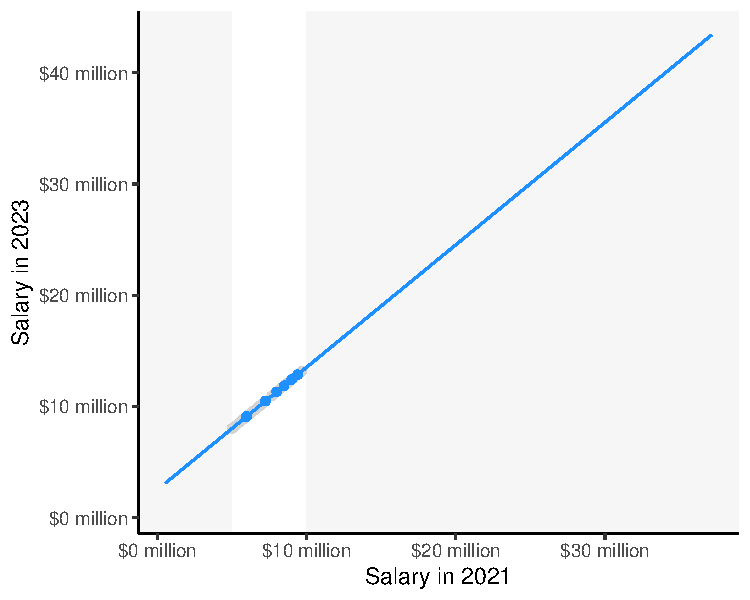
\includegraphics[width = .6\textwidth]{sims/ols_predicted_2}};
\node<5-6>[anchor = north west] (predict) at (0,.9) {Predict};
\node<6>[anchor = north east] at (1,.9) {Record the average};
\node<1-5>[anchor = east] at (1,.5) {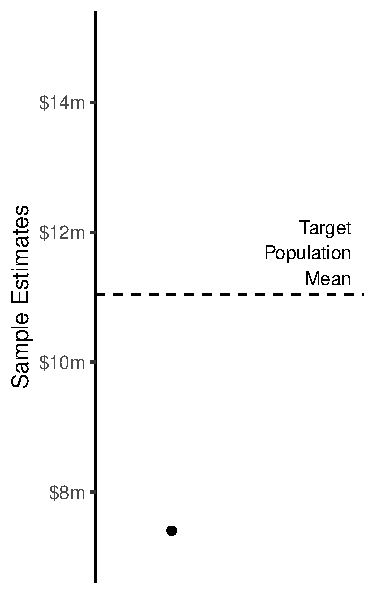
\includegraphics[width = .3\textwidth]{sims/ols_estimate_1}};
\node<6>[anchor = east] at (1,.5) {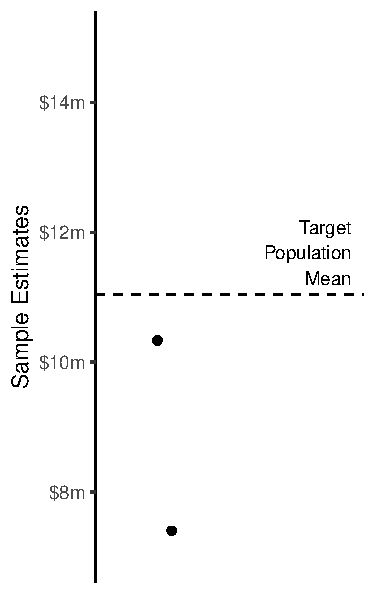
\includegraphics[width = .3\textwidth]{sims/ols_estimate_2}};
\end{tikzpicture}
\end{frame}

% OLS SAMPLE 3+
\begin{frame}{Goal: Estimate a target population mean from a sample}{Method: Ordinary Least Squares prediction}
\begin{tikzpicture}[x = \textwidth, y = \textheight]
\node at (0,0) {};
\node at (1,1) {};
\node[anchor = north west] at (0,.9) {Sample};
\node[anchor = north west] at (0,.5) {Learn};
\node[anchor = north east] at (1,.9) {Record};
\node<1>[anchor = west] at (.15,.8) {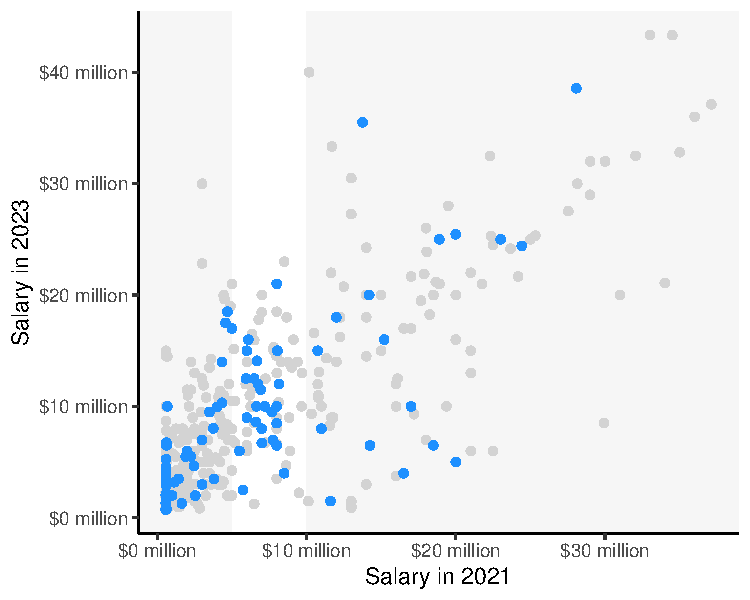
\includegraphics[width = .4\textwidth]{sims/sample_3}};
\node<2>[anchor = west] at (.15,.8) {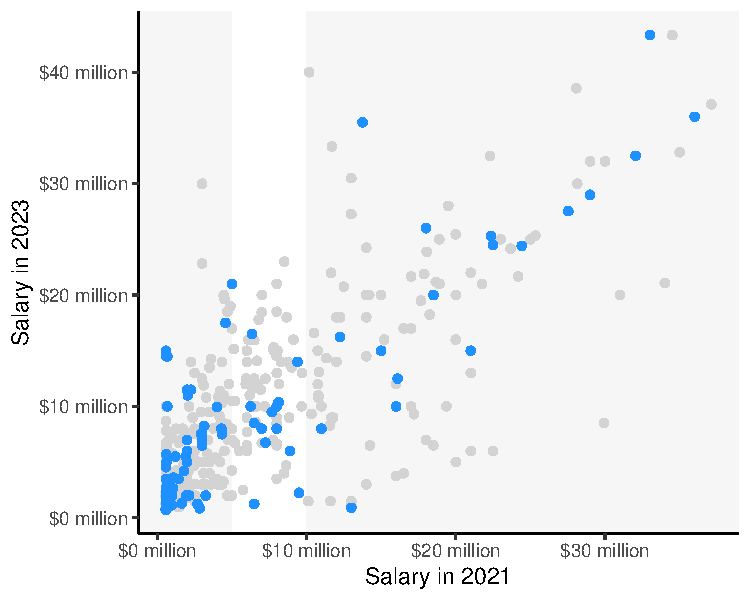
\includegraphics[width = .4\textwidth]{sims/sample_4}};
\node<3>[anchor = west] at (.15,.8) {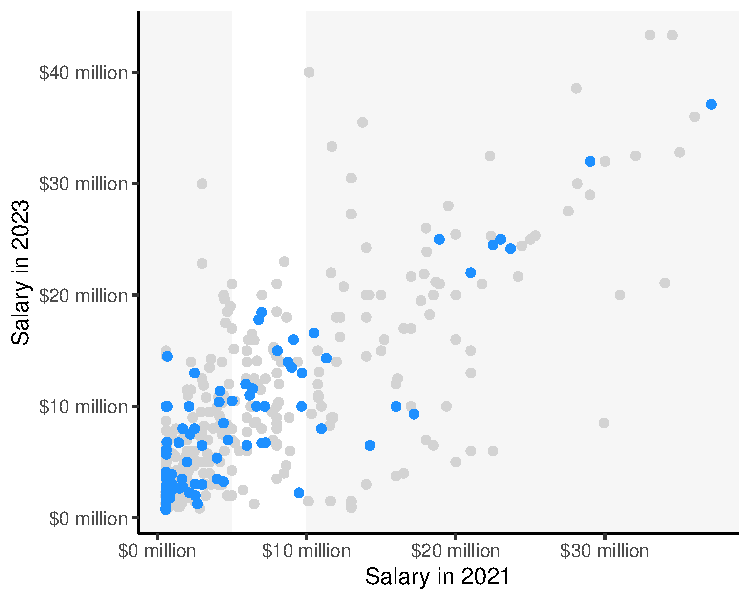
\includegraphics[width = .4\textwidth]{sims/sample_5}};
\node<4>[anchor = west] at (.15,.8) {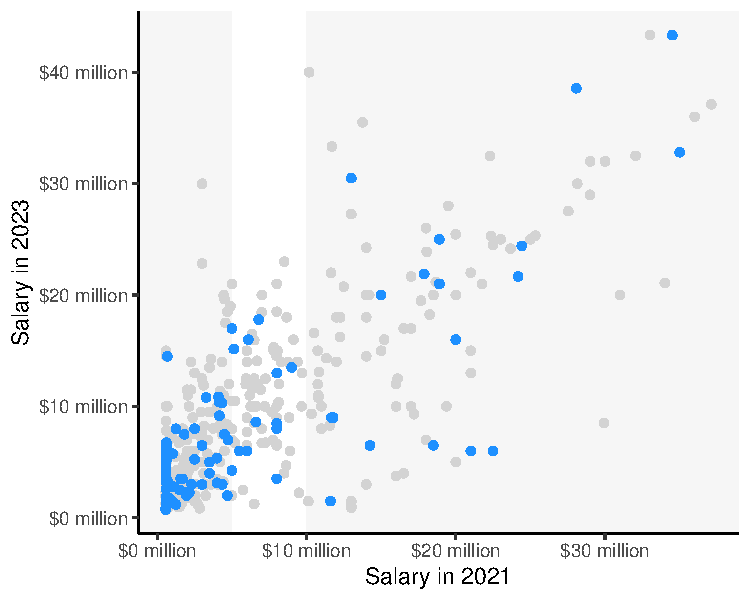
\includegraphics[width = .4\textwidth]{sims/sample_10}};
\node<5>[anchor = west] at (.15,.8) {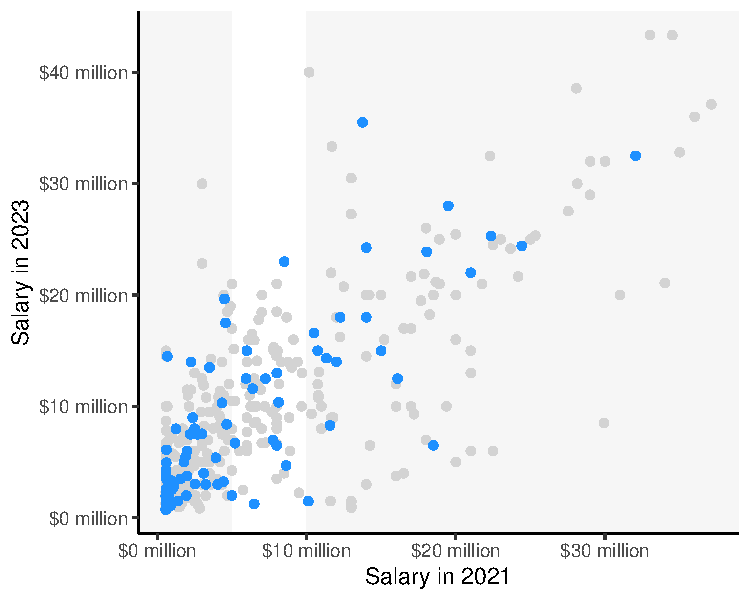
\includegraphics[width = .4\textwidth]{sims/sample_50}};
\node<6>[anchor = west] at (.15,.8) {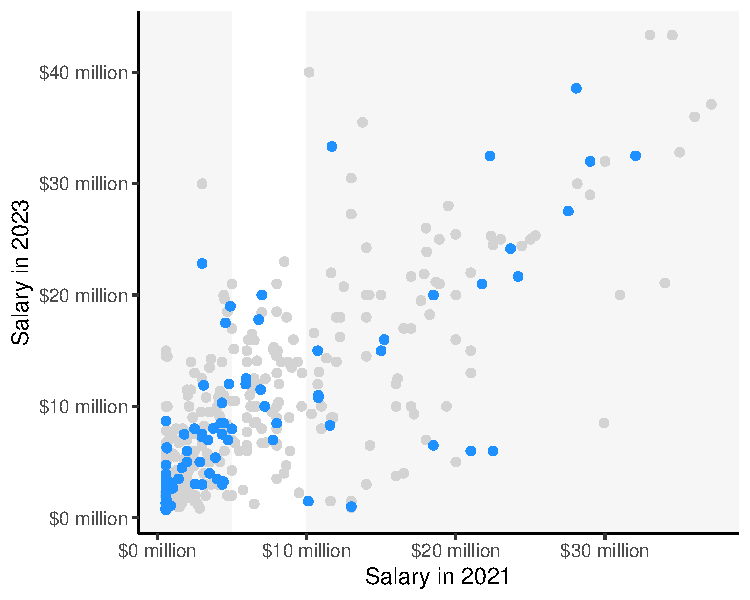
\includegraphics[width = .4\textwidth]{sims/sample_100}};
\node<1>[anchor = west] at (.15,.4) {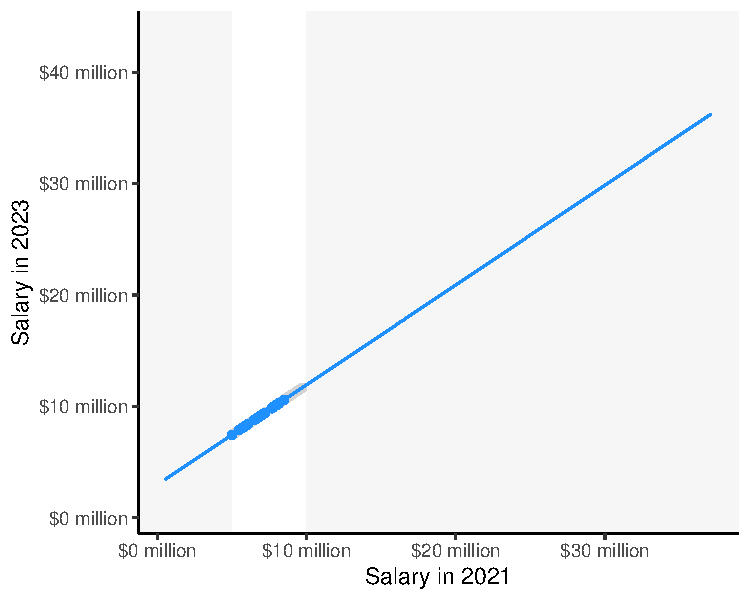
\includegraphics[width = .4\textwidth]{sims/ols_predicted_3}};
\node<2>[anchor = west] at (.15,.4) {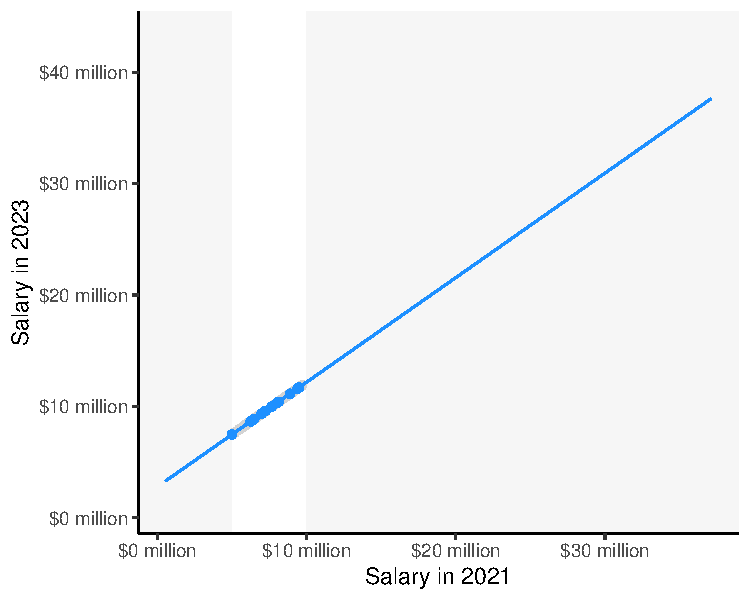
\includegraphics[width = .4\textwidth]{sims/ols_predicted_4}};
\node<3>[anchor = west] at (.15,.4) {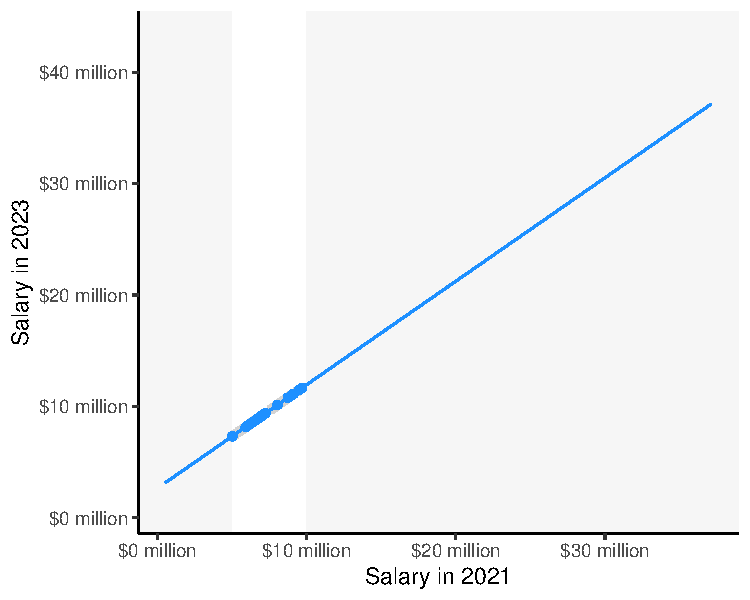
\includegraphics[width = .4\textwidth]{sims/ols_predicted_5}};
\node<4>[anchor = west] at (.15,.4) {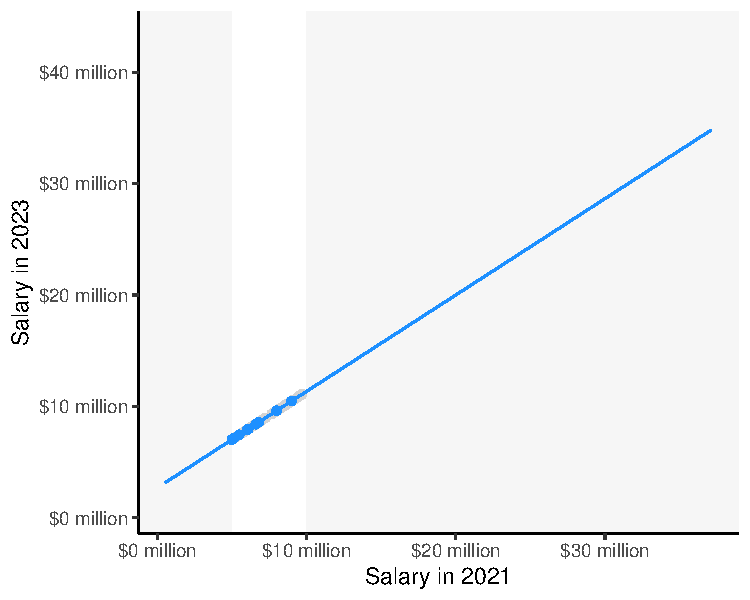
\includegraphics[width = .4\textwidth]{sims/ols_predicted_10}};
\node<5>[anchor = west] at (.15,.4) {\includegraphics[width = .4\textwidth]{sims/ols_predicted_50}};
\node<6>[anchor = west] at (.15,.4) {\includegraphics[width = .4\textwidth]{sims/ols_predicted_100}};
\node<1>[anchor = east] at (1,.5) {\includegraphics[width = .3\textwidth]{sims/ols_estimate_3}};
\node<2>[anchor = east] at (1,.5) {\includegraphics[width = .3\textwidth]{sims/ols_estimate_4}};
\node<3>[anchor = east] at (1,.5) {\includegraphics[width = .3\textwidth]{sims/ols_estimate_5}};
\node<4>[anchor = east] at (1,.5) {\includegraphics[width = .3\textwidth]{sims/ols_estimate_10}};
\node<5>[anchor = east] at (1,.5) {\includegraphics[width = .3\textwidth]{sims/ols_estimate_50}};
\node<6>[anchor = east] at (1,.5) {\includegraphics[width = .3\textwidth]{sims/ols_estimate_100}};
\end{tikzpicture}
\end{frame}

\begin{frame}

Ordinary Least Squares strategy:
\begin{enumerate}
\item Sample from the population
\item Learn a model
\item Record the average prediction in the target subgroup
\end{enumerate}

\end{frame}

\begin{frame}{Goal: Estimate a target population mean from a sample}

How would you do this with machine learning?

\includegraphics[width = .8\textwidth]{sims/gam_fit_1}

\end{frame}

% gam SAMPLE 1
\begin{frame}{Goal: Estimate a target population mean from a sample}{Method: Generalized Additive Model prediction}
\begin{tikzpicture}[x = \textwidth, y = \textheight]
\node at (0,0) {};
\node at (1,1) {};
\node<1>[anchor = north west] at (0,.9) {Begin with the population};
\node<1>[anchor = west] at (0,.5) {\includegraphics[width = .6\textwidth]{sims/population}};
\node<2>[anchor = north west] at (0,.9) {Draw a sample};
\node<2>[anchor = west] at (0,.5) {\includegraphics[width = .6\textwidth]{sims/sample_1}};
\node<3>[anchor = north west] at (0,.9) {Learn a model};
\node<3>[anchor = west] at (0,.5) {\includegraphics[width = .6\textwidth]{sims/gam_fit_1}};
\node<4>[anchor = north west] at (0,.9) {Focus on the target population};
\node<4>[anchor = west] at (0,.5) {\includegraphics[width = .6\textwidth]{sims/gam_target_1}};
\node<5-6>[anchor = west] at (0,.5) {\includegraphics[width = .6\textwidth]{sims/gam_predicted_1}};
\node<5-6>[anchor = north west] (predict) at (0,.9) {Predict};
\node<6>[anchor = north east] at (1,.9) {Record the average};
\node<6>[anchor = east] at (1,.5) {\includegraphics[width = .3\textwidth]{sims/gam_estimate_1}};
\end{tikzpicture}
\end{frame}
% gam SAMPLE 2
\begin{frame}{Goal: Estimate a target population mean from a sample}{Method: Generalized Additive Model prediction}
\begin{tikzpicture}[x = \textwidth, y = \textheight]
\node at (0,0) {};
\node at (1,1) {};
\node<1>[anchor = north west] at (0,.9) {Begin with the population};
\node<1>[anchor = west] at (0,.5) {\includegraphics[width = .6\textwidth]{sims/population}};
\node<2>[anchor = north west] at (0,.9) {Draw a sample};
\node<2>[anchor = west] at (0,.5) {\includegraphics[width = .6\textwidth]{sims/sample_2}};
\node<3>[anchor = north west] at (0,.9) {Learn a model};
\node<3>[anchor = west] at (0,.5) {\includegraphics[width = .6\textwidth]{sims/gam_fit_2}};
\node<4>[anchor = north west] at (0,.9) {Focus on the target population};
\node<4>[anchor = west] at (0,.5) {\includegraphics[width = .6\textwidth]{sims/gam_target_2}};
\node<5-6>[anchor = west] at (0,.5) {\includegraphics[width = .6\textwidth]{sims/gam_predicted_2}};
\node<5-6>[anchor = north west] (predict) at (0,.9) {Predict};
\node<6>[anchor = north east] at (1,.9) {Record the average};
\node<1-5>[anchor = east] at (1,.5) {\includegraphics[width = .3\textwidth]{sims/gam_estimate_1}};
\node<6>[anchor = east] at (1,.5) {\includegraphics[width = .3\textwidth]{sims/gam_estimate_2}};
\end{tikzpicture}
\end{frame}

% gam SAMPLE 3+
\begin{frame}{Goal: Estimate a target population mean from a sample}{Method: Generalized Additive Model prediction}
\begin{tikzpicture}[x = \textwidth, y = \textheight]
\node at (0,0) {};
\node at (1,1) {};
\node[anchor = north west] at (0,.9) {Sample};
\node[anchor = north west] at (0,.5) {Learn};
\node[anchor = north east] at (1,.9) {Record};
\node<1>[anchor = west] at (.15,.8) {\includegraphics[width = .4\textwidth]{sims/sample_3}};
\node<2>[anchor = west] at (.15,.8) {\includegraphics[width = .4\textwidth]{sims/sample_4}};
\node<3>[anchor = west] at (.15,.8) {\includegraphics[width = .4\textwidth]{sims/sample_5}};
\node<4>[anchor = west] at (.15,.8) {\includegraphics[width = .4\textwidth]{sims/sample_10}};
\node<5>[anchor = west] at (.15,.8) {\includegraphics[width = .4\textwidth]{sims/sample_50}};
\node<6>[anchor = west] at (.15,.8) {\includegraphics[width = .4\textwidth]{sims/sample_100}};
\node<1>[anchor = west] at (.15,.4) {\includegraphics[width = .4\textwidth]{sims/gam_predicted_3}};
\node<2>[anchor = west] at (.15,.4) {\includegraphics[width = .4\textwidth]{sims/gam_predicted_4}};
\node<3>[anchor = west] at (.15,.4) {\includegraphics[width = .4\textwidth]{sims/gam_predicted_5}};
\node<4>[anchor = west] at (.15,.4) {\includegraphics[width = .4\textwidth]{sims/gam_predicted_10}};
\node<5>[anchor = west] at (.15,.4) {\includegraphics[width = .4\textwidth]{sims/gam_predicted_50}};
\node<6>[anchor = west] at (.15,.4) {\includegraphics[width = .4\textwidth]{sims/gam_predicted_100}};
\node<1>[anchor = east] at (1,.5) {\includegraphics[width = .3\textwidth]{sims/gam_estimate_3}};
\node<2>[anchor = east] at (1,.5) {\includegraphics[width = .3\textwidth]{sims/gam_estimate_4}};
\node<3>[anchor = east] at (1,.5) {\includegraphics[width = .3\textwidth]{sims/gam_estimate_5}};
\node<4>[anchor = east] at (1,.5) {\includegraphics[width = .3\textwidth]{sims/gam_estimate_10}};
\node<5>[anchor = east] at (1,.5) {\includegraphics[width = .3\textwidth]{sims/gam_estimate_50}};
\node<6>[anchor = east] at (1,.5) {\includegraphics[width = .3\textwidth]{sims/gam_estimate_100}};
\end{tikzpicture}
\end{frame}

\begin{frame}{Comparing the estimators}
\begin{tikzpicture}[x = \textwidth, y = \textheight]
\node at (0,0) {};
\node at (1,1) {};
\onslide<1-5>{
\node[anchor = north west, align = left] at (0,1) {\includegraphics[width = .33\textwidth]{sims/sample_100}};
\node[anchor = north west, align = left] at (.3,1) {\includegraphics[width = .33\textwidth]{sims/ols_fit_100}};
\node[anchor = north west, align = left] at (.6,1) {\includegraphics[width = .33\textwidth]{sims/gam_fit_100}};
}
\node[anchor = south west] at (0,.2) {\includegraphics[width = .25\textwidth]{sims/mean_estimate_100}};
\node[anchor = south west] at (.3,.2) {\includegraphics[width = .25\textwidth]{sims/ols_estimate_100}};
\node[anchor = south west] at (.6,.2) {\includegraphics[width = .25\textwidth]{sims/gam_estimate_100}};
\onslide<2->{
\node[font = \footnotesize] at (.5,.22) {Variance};
\draw[<->, thick] (.47,.28) -- (.47,.42);
\node[font = \footnotesize, anchor = west] at (.5,.4) {Bias};
\draw[->, thick] (.5,.44) -- (.5,.36);
}
\node<3->[gray,  font = \footnotesize] (theta) at (.48,.52) {$\theta$};
\draw<3->[->, gray] (theta) to[bend right] (.45,.45);
\node<4->[gray, font = \footnotesize] (hat) at (.4,.2) {$\hat\theta$};
\draw<4->[->, gray] (hat) to[bend left] (.42,.267);
\node<5->[gray] at (.5,.35) {$\bullet$};
\node<5->[gray, anchor = west, font = \footnotesize] at (.52,.3) {$\E(\hat\theta)$};
\draw<5->[->, gray] (.55,.315) to[bend right] (.51,.35);
% Initial equation
\onslide<6>{
\node at (.1,.85) {$\left(\hat\theta - \theta\right)$};
\node at (.25, .85) {$=$};
\node at (.45,.85) {$\left(\hat\theta - \E\left(\hat\theta\right)\right)$};
\node at (.62, .85) {$+$};
\node at (.8,.85) {$\left(\E\left(\hat\theta\right) - \theta\right)$};
}
% Squared
\onslide<7>{
\node at (.1,.85) {$\left(\hat\theta - \theta\right)^2$};
\node at (.25, .85) {$=$};
\node at (.45,.85) {$\left(\hat\theta - \E\left(\hat\theta\right)\right)^2$};
\node at (.62, .85) {$+$};
\node at (.8,.85) {$\left(\E\left(\hat\theta\right) - \theta\right)^2$};
\node at (.43, .75) {$+$};
\node at (.7,.75) {$2\left(\hat\theta - \E\left(\hat\theta\right)\right)\left(\E\left(\hat\theta\right) - \theta\right)$};
}
% Expected
\onslide<8->{
\node at (.1,.85) {$\E\left[\left(\hat\theta - \theta\right)^2\right]$};
\node at (.25, .85) {$=$};
\node at (.45,.85) {$\E\left[\left(\hat\theta - \E\left(\hat\theta\right)\right)^2\right]$};
\node at (.62, .85) {$+$};
\node at (.8,.85) {$\E\left[\left(\E\left(\hat\theta\right) - \theta\right)^2\right]$};
\node<8-9> at (.43, .75) {$+$};
\node<8-9> (zero) at (.7,.75) {$2\E\left[\left(\hat\theta - \E\left(\hat\theta\right)\right)\left(\E\left(\hat\theta\right) - \theta\right)\right]$};
\draw<9>[thick] (zero.west) -- (zero.east);
\node<9>[anchor = west] at (zero.east) {=0};
}
\node<10>[align = center, anchor = north, font = \small] at (.1,.78) {Mean Squared\\Error};
\node<10>[anchor = north, font = \small] at (.45,.78) {Variance};
\node<10>[anchor = north, font = \small] at (.8,.78) {$\text{Bias}^2$};
\end{tikzpicture}
\end{frame}

\section{imperfect models}

\begin{frame}

{
\huge working with imperfect models
} \vskip .5in
Drawing on Berk 2020.\\\bref{https://link.springer.com/book/10.1007/978-3-030-40189-4}{\textit{Statistical Learning from a Regression Perspective}}

\end{frame}

\begin{frame}

\includegraphics[width = \textwidth]{dodger_model_wrong} \pause \vskip .1in

The model is wrong. Why might we still use it?

\end{frame}

\begin{frame}

\includegraphics[width = \textwidth]{berk_fig1.6.pdf}

\end{frame}

\goalsframe

\end{document}
